% This is lnicst.tex the demonstration file of the LaTeX macro package for
% Lecture Notes of the Institute for Computer Sciences, Social-Informatics 
% and Telecommunications Engineering series from Springer-Verlag.
% It serves as a template for authors as well.
% version 1.0 for LaTeX2e
%
\documentclass[lnicst,a4paper]{svmultln}
%
\usepackage[english]{babel}
\selectlanguage{english}
%
\usepackage{graphicx}
\DeclareGraphicsExtensions{.pdf,.svg,.jpg,.png,.eps} % first try pdf, then eps, png and jpg
%
\usepackage{makeidx}  % allows for indexgeneration
% \makeindex          % be prepared for an author index
%
\begin{document}
%
\mainmatter              % start of the contribution
%
\title{Humanoid robot obstacle recognition via data filtering, localisation and robot-to-robot communication in context of RoboCup} 
%
\titlerunning{Humanoid robot obstacle recognition}  % abbreviated title (for running head)
%                                     also used for the TOC unless
%                                     \toctitle is used
%
\author{Benjamin Scholz \and Daniel Speck \and Judith Hartfill}
%
\authorrunning{Benjamin Scholz \and Daniel Speck \and Judith Hartfill}   % abbreviated author list (for running head)
%
%%%% list of authors for the TOC (use if author list has to be modified)
\tocauthor{}
%
\institute{University of Hamburg, Fachbereich Informatik\\
\email{2scholz@informatik.uni-hamburg.de, 2speck@informatik.uni-hamburg.de, 2hartfil@informatik.uni-hamburg.de}
}

\maketitle              % typeset the title of the contribution
% \index{Ekeland, Ivar} % entries for the author index
% \index{Temam, Roger}  % of the whole volume
% \index{Dean, Jeffrey}




%%%%%%%%%%%%%%%%
%%%          %%%
%%% Abstract %%%
%%%          %%%
%%%%%%%%%%%%%%%%

\begin{abstract}        % give a summary of your paper
The abstract should summarize the contents of the paper. It will be set in 9-point
font size and be inset 1.0 cm from the right and left margins.
There will be two blank lines before and after the Abstract.

Use the abstract section to provide a teaser for the contents of your report I Do not attempt to write a review or summary I Be concise: Your abstract should have 200 words or less (do
not use more than 250 words)
%                         please supply keywords within your abstract
\keywords {obstacle recognition, obstacle avoidance, localisation, filtering, data smoothing, vision, swarm intelligence}
\end{abstract}
%




%%%%%%%%%%%%%%%%%%%%
%%%              %%%
%%% Introduction %%%
%%%              %%%
%%%%%%%%%%%%%%%%%%%%

\section{Introduction}
 
 
In this project our aim was to improve the way the robots are playing football together. Until then, each robot had its own view/opinion of the surrounding field and so was able to make decisions only due to this information. Our idea was to build an intern team communication system, that provides one robots information for every team member. Thus a form of swarm intelligence could increase the quality of the robots   acting together as a whole team. Considering that, it was necessary to develop a world model to make the information transfomable, unique and easy to provide. Furthermore we detected, that the image prosessing quality was not good enough to precisly determine the robots position and so we did some vision modifications and added some filters. 


Outline of underlying concepts

Brief summary of relevant theoretical background knowledge

Review of existing (published) work relevant for your topic(s)

Motivate the reader for the issue(s) you are trying to solve

Explain why your work (your approach) is necessary




%%%%%%%%%%%%%%%%%%
%%%            %%%
%%% Motivation %%%
%%%            %%%
%%%%%%%%%%%%%%%%%%

\subsection{Motivation}
Obstacle recognition and dynamis behaviour towards this is very important if several robots shall act together in a certain way. One of the main reasons for this is to avoid the physical contact between robots. As long as their hardware is not good enough to hold balance when beeing touched, they are very likely to fall and - in worst-case-scenario - bring about anothers robots downfall. This usually causes hight costs for hardware fixes and also disturbs the gameplay. Getting up again can take several seconds and toward the opposite robots it is not within the meaning of fairplay.
Besides more and especially better knowledge about the surroundings is strategically important in the RoboCup competition. Having a reliably prospect of its own positions, the position of the ball and the opposites robots position combined with a good path finding algorithm can raise the number of scores significantly.
was war das problem bisher?




%%%%%%%%%%%%%%%%
%%%          %%%
%%% Problems %%%
%%%          %%%
%%%%%%%%%%%%%%%%

\subsection{Problems}

\subsubsection{Vision}
When we checked how good the already implemented algorithm worked we discovered, that ot even the goals were recognized suffinciently. The kind of jumoed from one point to the other and most of the time their were more than two goal postst recognized fo one goal. In addition obstacles at least could be recognise, but there was no behaviour to react in a senseful way. Moreover it was no possible for the robot to distinguish between obstacles, such as team mate or opposite player.

\subsubsection{Filtering}
The whole topic of obstacle recognition relies on information which is extracted out of (heavily) noisy input data.
\\
For our solutions primarily the goal post data and the later calculated goal center information is important, 
\\
Since the robots do not have auto-calibration features the calibration of the camera and motor angles deteriorate the noise problem because once the calibration is manually done its configuration is static but the real values vary other time, for example when the robot falls accidently.
\\
In addition to that the manual calibration is expansive in terms of time.




%%%%%%%%%%%%%%%%%
%%%           %%%
%%% Solutions %%%
%%%           %%%
%%%%%%%%%%%%%%%%%

\section{Solutions}
What did you do and how did you do it?

Methods

Design

Implementation

Do not include every possible detail and avoid redundancy

Use subsections to emphasize certain aspects/components of
your work -
but do not overuse them!

Avoid the passive voice: Y was done by X, use the active voice: X did Y




%%%%%%%%%%%%%%
%%%        %%%
%%% Vision %%%
%%%        %%%
%%%%%%%%%%%%%%

\subsection{Vision}




%%%%%%%%%%%%%%%%%
%%%           %%%
%%% Filtering %%%
%%%           %%%
%%%%%%%%%%%%%%%%%

\subsection{Filtering}

\subsubsection{Data noise}
The majority of the bitbots code works without filters on raw data, especially in the case of goal information, which is needed to localise the robot on the field in our case, no data postprocessing exists.

\subsubsection{DBSCAN} Our approach to reduce the noise on data was implementing a two dimensional version of the DBSCAN (density-based scanning) algorithm \cite{ester:kriegel}, which we slightly customized to our needs.
\\
At first our code was an exact re-implementation in pure Python of the DBSCAN algorithm \cite{ester:kriegel}
originally proposed by Martin Ester et al. in 1996 but this procedure was just for testing to ensure the algorithm meets our requirements.
\\
Due to the performance issues of pure Python implementations we refactored the complete code and made use of Numpy (mainly) and other SciPy libraries. As a consequence of the C/C++ core implementations of those libraries the overall execution time of our code decreased.
\\
In addition to that the refactored, performant version of our DBSCAN is implemented object oriented. This leads to an overhead in space complexity but offered easier debugging as well as an additional improvement of execution time because the calculations are saved in objects and those cached results are re-used as much as possible.
\\
In our tested cases the pure Python implementation ran about 8 - 12 times slower on average (dependent on current background tasks) on our darwin-op hardware compared to our current object oriented Python implementation with Numpy and other SciPy libraries.
\\
Those optimizations are essential considering the very limited computing power of our current darwin-op robots.
\\
For calculating the goal information each goal posts raw input data (if post is seen) is recorded separately in buffers of a maximum size of 60 items on every new frame. If a buffer is full, the oldest entry is dropped and the newest saved. As data structure for the buffers we chose Python Deque objects.
\\
If the robot changes its position, old data sets would mess up the calculation, so our DBSCAN object automatically drops data sets which are older than 10 seconds to prevent those kind of failures. Minor positional changes in the meantime are no problems in most cases, because the DBSCAN would filter those datasets appropriately.
\\
In figure~\ref{fig:dbscan1} a graphical illustration of the DBSCAN algorithm
is shown.

\begin{figure}
 	\centerline{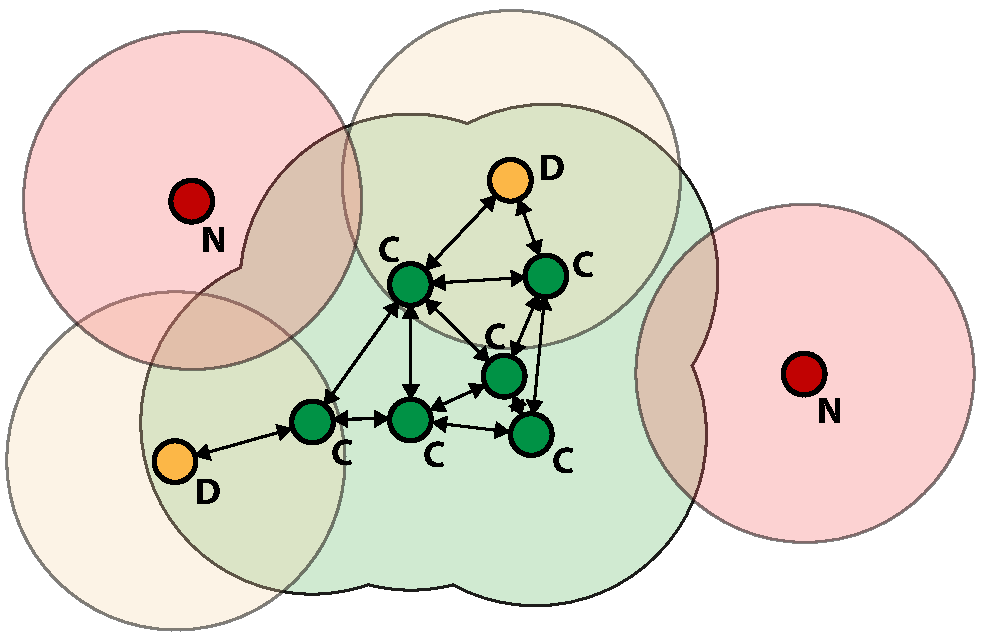
\includegraphics[width=0.7\textwidth]{dbscan1.pdf}}
	{\caption{DBSCAN graphical illustration.
	The points labeled with `C' are core points,
	the yellow ones labeled with `D' are density-reachable points
	and the red ones labeled with `N' noise points.
	The minimum points parameter is set to $4$ in this example.}\label{fig:dbscan1}}
\end{figure}

Throughout our testing process we experienced positive results with 6 minimum points and an epsilon of 50 as parameters for our DBSCAN implementation.




%%%%%%%%%%%%%%%%%%%%
%%%              %%%
%%% Localisation %%%
%%%              %%%
%%%%%%%%%%%%%%%%%%%%

\subsection{Localisation}

\subsubsection{Calculating the position of a robot}
We didn't have a lot of data to work with. The only data that we could use were the distances to the goal and to the goalposts. There is a lot of other data: like already mentioned the distance to obstacles or other players on the field and the distance to the ball. But the problem with those is that they are not a fixed point on the field. They will change their position and that means they are not suitable to calculate our own position. Or more accurately the distance in front and the distance to the left which depends on the direction of the robot. We will call the distance in front of him u and to the left of him v to stay consistent with the terms used in the code. The following graphic shows what these values are:\\
insert graphic of U and V values\\
With these values it's easy to calculate the direct distance to the goal. You can use Pythagora's theorem to do that: \(d = \sqrt{u^2+v^2}\)\\
We do that for both goal posts. The size of the field and the goal are known beforehand, so we can use the width of the goal as well. With these three values we can build a triangle:\\
triangle graphic\\
With the help of that triangle we are going to calculate the point of intersection of d1 and d2. Let's assume that we have a coordinate system and the point of origin is at the middle of the field. The reason for that is that the origin of our grid world, that is used to save the data, is in the middle of the field too. That means it's easier to translate the position found in that coordinate system to the grid world. But we will explain that in the next section. Otherwise it would have been easier to have the origin in the middle of the goal the robot is facing to. To calculate the point of intersection we need to know the slope of both lines. We can use the angles in the triangle for this purpose:\\
Vielleicht Grafik\\
The formula we used is the following: \(\arccos{(\frac{a^2-b^2-c^2}{-2bc})} = \alpha\)\\ Specifically these are the two formulas if you want to calculate the angle from the left post and the right post in the triangle:\\ 
\(angleleft = \arccos{\frac{(d1^2 - d2^2 - goalwidth^2)}{(-2*d2*goalwidth)}}\)\\
\(angleright = \arccos{\frac{(d2^2 - d1^2 - goalwidth^2)}{(-2*d1*goalwidth)}}\)\\
Now we know the two angles in the triangle. To convert the angles to the slopes in the coordinate system we can do the following:\\
\(slopeleft = \frac{1}{\tan{angleleft}}\)\\
On the right side we don't need the angle itself but 180 minus the angle:
\(sloperight = \frac{1}{\tan{180 - angleright}}\)\\
Because we want to know the point of intersection of these two lines we need an equation for them:\\
\(y = slopeleft * x + b1\)\\
\(y = sloperight * x + b2\)\\




%%%%%%%%%%%%%%%%%%
%%%            %%%
%%% Grid World %%%
%%%            %%%
%%%%%%%%%%%%%%%%%%

\subsubsection{Grid World}
Now that we know where our own robot stands we need some way to share the position, so that our team mates can use that knowledge and every robot in our team can profit. For that purpose we use the grid world. We needed a representation of the field, so we could safe and use the data we generated. There are different approaches for that. Other approaches that we considered were a coordinate system that uses millimetres and tree based solution. In the end we decided to use said grid world. For that we divided the field in certain number of cells. The origin of those cells is in the middle of the field:\\
grid world grafik\\
We had different iterations of the grid world with different origins. At first the origin cell was in the lower left corner. Then we decided it would be better if the origin cell were in the middle of the own goal, mostly because it made calculations needed to determine the position of the robots easier. But if we wanted to use these calculations for the opponents goal too, it is easier to have the origin cell in the middle. There is also a difference between choosing an even number and uneven number respectively on the x and the y direction. We decided to choose an uneven number for both, which means the origin cell is now in the middle of the centre spot. One benefit of that is that there is a cell that is in the middle of the goal where the goalie can stand. When we take the cell at position (0,0) for example and we compare it to a coordinate system, then the upper right edge of that cell would be at (0.5, 0.5) in the coordinate system. When we calculate positions we don't get integers but decimal digits. So if it is over 0.5 instead of the cell with the 0 position we will put it in the cell with the position 1. 
For that purpose we used a dictionary in Python. We used numbers to fill that dictionary. At initialization the dictionary will be filled with zeroes, which is representing that there is nothing at that particular position. Here is a quick overview of the numbers we fill the dictionary with and what they represent:\\
0: nothing\\
1: own goal\\
2: enemy goal\\
3: own position\\
4: team mate\\
5: opponent\\
6: unclassified obstacle\\
Every robot can determine their own position themselves. The position of the team mates is shared over the wifi, which will be explained in the next section. The robots can determine the position of opponents that they see. They share those positions so everyone has the position of as many opponents as possible. The robots actually can't distinguish between team mate and opponent. But because we know all the positions of our team mates the robots can compare the position of the robots they see with the position of their team mates in their grid world. Only if there isn't a team mate in that cell they will identify the robot as an opponent. Another problem is to keep the map up-to-date. We send the whole map over the wifi, so it would be possible to check if there still is a robot on a certain position when the robot looks in that direction. Another solution would be to delete the positions of the opponents after a certain amount of time. There is the same problem with team mates. Currently we don't send which team mate shares the position, but that would be one solution. Whenever a team mate shares their new position a the receiving robot could delete the old position.\\




%%%%%%%%%%%%%%%%%%%%%
%%%               %%%
%%% Communication %%%
%%%               %%%
%%%%%%%%%%%%%%%%%%%%%

\subsection{Communication}




%%%%%%%%%%%%%%%
%%%         %%%
%%% Results %%%
%%%         %%%
%%%%%%%%%%%%%%%

\section{Results}
Present your results in a logical sequence

Highlight the importance of your results and explain your
analysis methodology

Discuss the results you infer from your work

Important:
Adopt a critical approach in your discussion

Do not oversell your results - put the advantages first, but
don’t forget to mention the shortcomings!




%%%%%%%%%%%%%%%
%%%         %%%
%%% Summary %%%
%%%         %%%
%%%%%%%%%%%%%%%

\section{Summary}

Be more informative than your abstract!

Include a concise version of your discussion

Highlight what you found out

Highlight the problems you encountered

Explain how your results support your conclusions!

Provide suggestions for future research and briefly outline how
suggested research can be attempted

Important:
Make this section readable




%%%%%%%%%%%%%%%%%%
%%%            %%%
%%% References %%%
%%%            %%%
%%%%%%%%%%%%%%%%%%

\section{References}
Very important section of your report

If you used external information/results
)
Provide a
reference!

References will help the reader understand the basis of your
work and provide context for comparison

Use of references might also help you to be more concise

There are several types of reference

Book

Journal article

Conference publication

Web site

Web sites are usually unchecked sources -
be careful




%%%%%%%%%%%%%%%%%%%%%%%%%%
%%%                    %%%
%%% Notes and Comments %%%
%%%                    %%%
%%%%%%%%%%%%%%%%%%%%%%%%%%

\paragraph{Notes and Comments.}
The first results on subharmonics were
obtained by Foster and Kesselman in \cite{fos:kes}, who showed the existence of
infinitely many subharmonics both in the subquadratic and superquadratic
case, with suitable growth conditions on $H'$. Again the duality
approach enabled Foster and Waterman in \cite{fos:kes:2} to treat the
same problem in the convex-subquadratic case, with growth conditions on
$H$ only.

Recently, Smith and Waterman (see \cite{smit:wat} and May et al. \cite{mes})
have obtained lower bound on the number of subharmonics of period $kT$,
based on symmetry considerations and on pinching estimates, as in
Sect.~5.2 of this article.




%%%%%%%%%%%%%%%%%%%%
%%%              %%%
%%% Bibliography %%%
%%%              %%%
%%%%%%%%%%%%%%%%%%%%

\begin{thebibliography}{5}

\bibitem{ester:kriegel} Ester, M., Kriegel, H.-P., Sander, J., Xu, X.:
A Density-Based Algorithm for Discovering Clusters in Large Spatial Databases with Noise.
In: Proceedings of 2nd International Conference on Knowledge Discovery and Data Mining (KDD-96),
pp. 226--231. AAAI Press, Munich (1996)

\bibitem{smit:wat} Smith, T.F., Waterman, M.S.: Identification of Common Molecular
Subsequences. J. Mol. Biol. 147, 195--197 (1981)

\bibitem{mes} May, P., Ehrlich, H.C., Steinke, T.: ZIB Structure Prediction Pipeline:
Composing a Complex Biological Workflow through Web Services. In: Nagel,
W.E., Walter, W.V., Lehner, W. (eds.) Euro-Par 2006. LNCS, vol. 4128,
pp. 1148--1158. Springer, Heidelberg (2006)

\bibitem{fos:kes} Foster, I., Kesselman, C.: The Grid: Blueprint for a New Computing
Infrastructure. Morgan Kaufmann, San Francisco (1999)

\bibitem{cff} Czajkowski, K., Fitzgerald, S., Foster, I., Kesselman, C.: Grid
Information Services for Distributed Resource Sharing. In: 10th IEEE
International Symposium on High Performance Distributed Computing, pp.
181--184. IEEE Press, New York (2001)

\bibitem{fos:kes:2} Foster, I., Kesselman, C., Nick, J., Tuecke, S.: The Physiology of the
Grid: an Open Grid Services Architecture for Distributed Systems
Integration. Technical report, Global Grid Forum (2002)

\bibitem{url} National Center for Biotechnology Information, http://www.ncbi.nlm.nih.gov

\end{thebibliography}





\end{document}